\section{Background}
This section will present the framework of this paper. First, existing game genres in which Archipelago takes inspiration from, as well as what have been identified as their key patterns will be defined. This definition process is important as a pre-emptive work to understand the bases on which the project was created. 

This will lead to a comprehensive definition of \textit{hybrid games}, and an identification of their core aspects. Furthermore, an analysis of early experiments showing a growing interest for hybrid games will be provided; this will help understanding the challenges implied by the development of hybrid games, as well as why the hybrid concept only reaches a wide audience now. This segment will be concluded by a play-through analysis of a hybrid game that is already on the market.

Because PCG was chosen to support the core mechanics of Archipelago, defining this programming concept is, and explaining how it is traditionally used in game design will also be a crucial aspect of this section. An overview of the technical definitions will be provided, followed by a description of the concepts that are important when designing with PCG. 

To complete this framework and before proceeding to the project in itself, important design theories will be presented. Those concepts are essential to boil down the critical elements identified by the definition and analysis processes, and to properly understand how hybrid games should be thought and conceived.
\subsection{Tabletop game play as a social activity}
It is commonly admitted that there are as many definitions of games as there are players. People working in the game industry, researchers, and players still disagree on which key elements should a taxonomy of games be based on. The french sociologist Roger Caillois (2001, p.3)\cite{book:mpg} explains the difficulty of establishing an all-inclusive game classification:
\begin{quotation}
The multitude and infinite variety of games at first causes one to despair of discovering a principle of classification capable of subsuming them under a small number of well-defined categories. Games also possess so many different characteristics that many approaches are possible.
\end{quotation} 
With this statement, one could argue that defining or classifying game genres is not relevant, as there will always be examples that do not fit the definition, which will then need to be extended and will therefore move away from its original meaning. This paper will certainly not bring a clear and universal definition of the game genres relevant to its topic, as definitions and taxonomies are necessarily affected by their research purpose. Nonetheless, basic definitions are needed to construct an understandable framework and provide tools that will help analysing the impact of the use of PCG in tabletop games, both on their design and creation and on the experience they enable.\subsubsection{Tabletop Games}
The definition of \textit{tabletop games} is the first one that must be refined in order to correctly comprehend the purpose of this paper. An example is needed as a reference in order to point out their key aspects. Game Designer Nat Levan (Oakleaf Games) gives his own definition of tabletop games. 
\begin{quotation}
The defining feature of a tabletop game is the need for components, not the need for a table. [...] [S]o perhaps saying that a tabletop game is a game with a structured placement of components establishes a better requirement (Levan, 2014)\cite{web:oak}.
\end{quotation}
\textit{Tabletop games} is a generic term used to refer to a broad variety of game genres that are played on a table or the like. They range from card games, board games, not forgetting miniature games or dice games. Although removing the need for a table from the definition seems rather counter-intuitive, this assumption is made to include other simple games using components. Nat Levan uses the example of the game of "guess what I'm holding in my hand"(Levan, 2014)\cite{web:oak} in order to justify his statement. Fully digital games are excluded from this range, although the line is sometimes thinner than one can imagine. The game \textit{Hearthstone: Heroes of Warcraft} (Blizzard Entertainment, 2014) for example, is a video game inspired from classical trading-card games\footnote{Card games in which players fight with decks of cards they collected and designed themselves.}. It uses the possibilities offered by digital devices to enhance a simulated tabletop experience: interactions with the surface on which the game is played, screaming voices to simulate an excited crowd watching the players or animations providing feedback when a card is played. The game goes far beyond what traditional trading-card games usually enable.

However, it seems that this approach is rather incomplete, because it overshadows the social aspect of tabletop games. It is understandable that tabletop games are not necessarily meant to gather people around a table to play. As an example, platforms allowing traditional tabletop games like \textit{Carcassone} (Wrede, 2000)\cite{game:carca}, \textit{Through the Ages: A Story of Civilization} (Chvátil, 2006)\cite{game:ages} or \textit{Race for the Galaxy}\ (Lehmann, 2007)\cite{game:race} and many others to be played online have made their appearance with the development of the internet. 
These games do not cease to be \textit{tabletop games} (even though the play experience is made different by changing the context in which they are played). This case is very particular though, as these online platforms solely propose an adaptation of already existing tabletop games, and do not use any advantages of digital devices to transform the games themselves, or create new ones. In that sense, it cannot be compared to a game that completely transforms the tabletop experience like \textit{Hearthstone: Heroes of Warcraft}.  However, this example really emphasizes a critical element defining tabletop games: these games need a space where the players can gather and participate to the play experience. In his work retracing the history of eurogames
\footnote{A particular type of tabletop game culture that has originated in Europe.}
, Stewart Woods (2012, p.212)\cite{book:euro} explains why the social aspect of tabletop games is a defining element:
\begin{quotation}
The play of tabletop games is a complex social activity.[...] [M]anagement of the immediate social setting in tabletop games adds a meta-level of understanding that cannot help but inform the process of play. The social context of the game can indeed shape play in a variety of ways, since players are always mindful of the social environment in which a game encounter takes place.
\end{quotation}
In consequence, the nature of tabletop games is what shapes the very particular play experience that they enable. Playing tabletop games means finding the right balance between being competitive and fair; and designing tabletop games also means supporting this shared experience and taking it into account. As long as they are made to be played by several players, tabletop games and their social dimension are inseparable (in the particular case of tabletop games meant to be played by only one player, this quality of tabletop games can be put aside).
\\\\
To complete the reflection, the next step of the process is to define what can be called \textit{components}, and why they have to be central in the case of tabletop games. Core components of tabletop games are generally thought as physical. They can be cards, tokens, pawns, dice or any object used as a core element in the game, which can therefore not be played without them. As is well known, tabletop games have generally evolved staying away from digital components. Exceptions exist though, and game makers have already experimented the use of technology to influence their design. The game \textit{Nightmare}\footnote{More generally known as \textit{Atmosfear} in the rest of the world, \textit{Nightmare} being the original title in the United States.} (Clements and Tanner, 1991)\cite{game:atmo} included a VHS tape showing "The Gatekeeper", who attributes rewards to the players, punishes them or gives them instructions at specific moments in the game, thus also acting as a timer. In that sense the VHS can be seen as a component in itself, like a deck of cards with a hourglass.

Components can then be defined as interactive elements without which the game cannot be played. The central dimension of components is clearly understandable, but it is important to notice that their physical property has been excluded from the definition.
\\\\
After these clarifications, it is now possible to come up with a definition of what tabletop games are. Tabletop games cannot be narrowed to the simple use of physical components, neither must they absolutely be played on a table; a more appropriate definition could be that tabletop games are games requiring the players to use their central components in a physical space in which player(s) gather, interact and participate to a social play experience. 
\subsubsection{Board Games}
\textit{Board games} are generally considered as a subcategory of tabletop games. Therefore, it can be acknowledged that the properties of board games derive from those of tabletop games. Oxford Dictionaries (2016)\cite{web:oxford} provide the following definition:
\begin{quotation}
"A game that involves the movement of counters or other objects round a board."
\end{quotation}
While this is a rather broad definition, it can still be used to present key aspects of board games. The terms "counters or other objects" refer to the core components that were previously mentioned as a key aspect of tabletop games. The new element here entering the definition being the game board, which is the surface on which the players move pieces, place cards or tiles in order to achieve the goal of the game. As it has been explained beforehand, this surface is not necessarily physical and can be then represented on a digital device like a screen. In a board game, the board is of course a key component. It is the center of the attention of players, and can serve several purposes.

The game board concentrates all the structural elements that the players should focus on in order to correctly play the game. It must support the play experience and also put limitations on the way the game is played. It that sense, it is as much an interface from which players extract the - more or less abstract - information they need, as it is an \textit{obstacle} forcing them to play according to the rules. In the game of \textit{Chess} for example, where planning and anticipation are the building blocks of the experience, those properties are clearly identifiable - though the board is not the most elaborate one. It limits the movement of the pieces within a square of 8 units of length, and a trained eye can easily identify valuable information (i.e. the movement possibilities), thanks to the tiled structure of the checker. 

One last property that can be identified, is that a board is rarely a core component in itself. During a game, the board only makes sense when it is accompanied by other core components like tokens or cards. Following the example of  \textit{Chess} again, the checker alone does not provide the necessary information in order to properly plan a strategy. It is only when the pieces are on the board that an experienced player can almost literally see the possible moves and anticipate the danger. This is only one example: game boards have different structures and purposes, and listing their properties here would not be relevant. But from those identified earlier, it becomes possible to give a definition of games using boards: \textit{board games} are tabletop games using a game board and its properties as a core component.
\subsubsection{Competition, collaboration and cooperation}
As Salen and Zimmerman explained (2003)\cite{book:rop}, "conflict" has clearly been identified as a defining element of games. Play enables a particular context in which conflict and the sense of achievement becomes the focus point of the experience. This particular context is what Salen and Zimmerman explain as a "magic circle" (Huizinga, 1938, cited in Salen and Zimmerman, 2003, pp. 94-95)\cite{book:rop}. It is a virtual space that is created by players in which all the participants agree to follow a certain set of rules that can be clearly identified (e.g. the rule book of a tabletop game) or unspoken (e.g. fair-play). While this is a metaphor that raises questions as much as it solves problems, it helps to understand why games can be thought as intrisically conflictual. Playing a game consists in a struggle towards the winning condition, which can of course take different forms. Trying to win is what provides a meaning to play in the first place, and all the potential experiences that appear while playing can be thought as a result of this race toward victory. Basing their reflection on this approach of game as system of conflicts, Salen and Zimmerman (2003, p.255)\cite{book:rop} explain the competitive dimension of games as follows:
\begin{quotation}
Our opinion is that all games are competitive. All games involve a conflict, whether that conflict occurs directly between players or whether players work together against the challenging activity presented by the game system.
\end{quotation}
This statement shows that competition must not be opposed to cooperation. While competition in games is traditionally  thought as a contest between players, it can also be considered as a struggle against the game. This is especially the case for single player games, in which the only obstacles that are placed on the player's way towards victory are set by the game itself. Competition is still present, and only its target changes. 

Yet, the authors do not make a distinction here between \textit{cooperating} and \textit{collaborating}. Though their respective approaches on the play experience can be expected to be similar, some researchers make the difference between cooperative and collaborative game play. Nash (2002, cited in Zagal and Rick, 2006, p.25)\cite{art:collab} argues that in cooperative games, the players have interests that are "neither completely opposed, nor completely coincident". In contrast, "in a collaborative game, all the participants work together as a team, sharing the pay-offs and outcomes; if a player wins or loses, everyone wins or loses"(Zagal and Rick, 2006, p.25)\cite{art:collab}. This differentiation between \textit{cooperation} and \textit{collaboration} makes a big difference in the play experience. As an example, \textit{Diplomacy} (Calhamer, 1959)\cite{game:diplo} encourages players to create alliances between them, and betray them when it is needed. On the other hand, in \textit{Forbidden desert} (Leacock, 2013)\cite{game:desert}, players have to manage the resources they individually possess and put their skills at the service of a team. 
This contrast is noticeable thanks to the interactions between the players. Collaboration involves more open discussions among the players and exclude the necessity to voluntarily hide information. Playing around this type of interactions outlines the tabletop game social play experience even more.
\subsection{Hybrid games}
\textit{Hybrid games} is an expression that has many different definitions, and the genre is still partially explored. Nonetheless, researchers have shown interest in this field and characteristics specific to hybrid games, derived from both tabletop and digital genres can be pointed out.
\subsubsection{Defining hybrid games}
There is not a universal understanding of what hybrid games are. Some people simply call \textit{hybrid games} games that are a combination, or hybridization, of two or more different genres of games. The interest of that definition is that it removes the analogue or digital aspect of games and simply focuses on the experience they provide. It needs to be refined though, because many games can be seen as a combination of genres, as game designers often build upon already existing game mechanics, trying to adapt them in another context. 

In this paper, \textit{hybrid games} are considered as a subcategory of tabletop games (and all their properties previously defined) using one or several digital components. They are based on the fact that players interact between each other by gathering around a space (like a board), and use the different components required to play the game in that space. The game structure has to support those interactions, thanks to its rules and mechanics. From that point of view, hybrid games are not that different from tabletop games - or even board games in some cases.

One criteria needs to be added though: as it has been already mentioned, the digital or analogue nature of the components does not change what defines tabletop or board games. Consequently, hybrid games must have another property. A game is much more than its components, game play mechanics or even its rules. De Boer and Lamers (2004, p.443)\cite{chap:aug} explain how the "possible electronic augmentation for board games" should be designed:

\begin{quotation}
[...] innovations should have a clear added value to the game concept and introduce new elements. Most importantly, the pleasure of playing a board game should be increased, while the existing physical elements of the game are preserved as much as possible. Summarizing, one could say that the added technology should fill holes in the game concept, that cannot be filled using traditional manners.
\end{quotation}

Therefore, only tabletop games including digital components in order to enable an experience that cannot exist without using the computing power of digital devices will be considered as \textit{hybrid games} in this paper. This aspect can of course take different forms depending on the game, like "randomly changing the board composition" or integrating "digital game rules" and "automatic error detection and prevention" (De Boer and Lamers, 2004, p.443)\cite{chap:aug}. Games that only use digital devices to simulate analogue game components (deck of cards or board for example) without providing any new feature are not considered hybrid games in this paper.

Another element must also be pointed out. Hybrid games are indeed a combination of patterns that can be found in digital games and in tabletop games. As such, their mechanic are in general not something new for an experience player of both digital and analogue games. However, the play experience delivered by this combination of patterns has to be original in its own way.
\subsubsection{A Hybrid Game Experiment: \textit{False Prophets}}
People have also started to refer to \textit{hybrid games} as games that try to close the gap between analogue and digital games. \textit{False Prophets} is an experimental game that explores "the space between board games and video games, leveraging the advantages of both" (Mandryk and Maranan, 2002)\cite{art:prophets}. 

\begin{figure}[h]
    \centering
    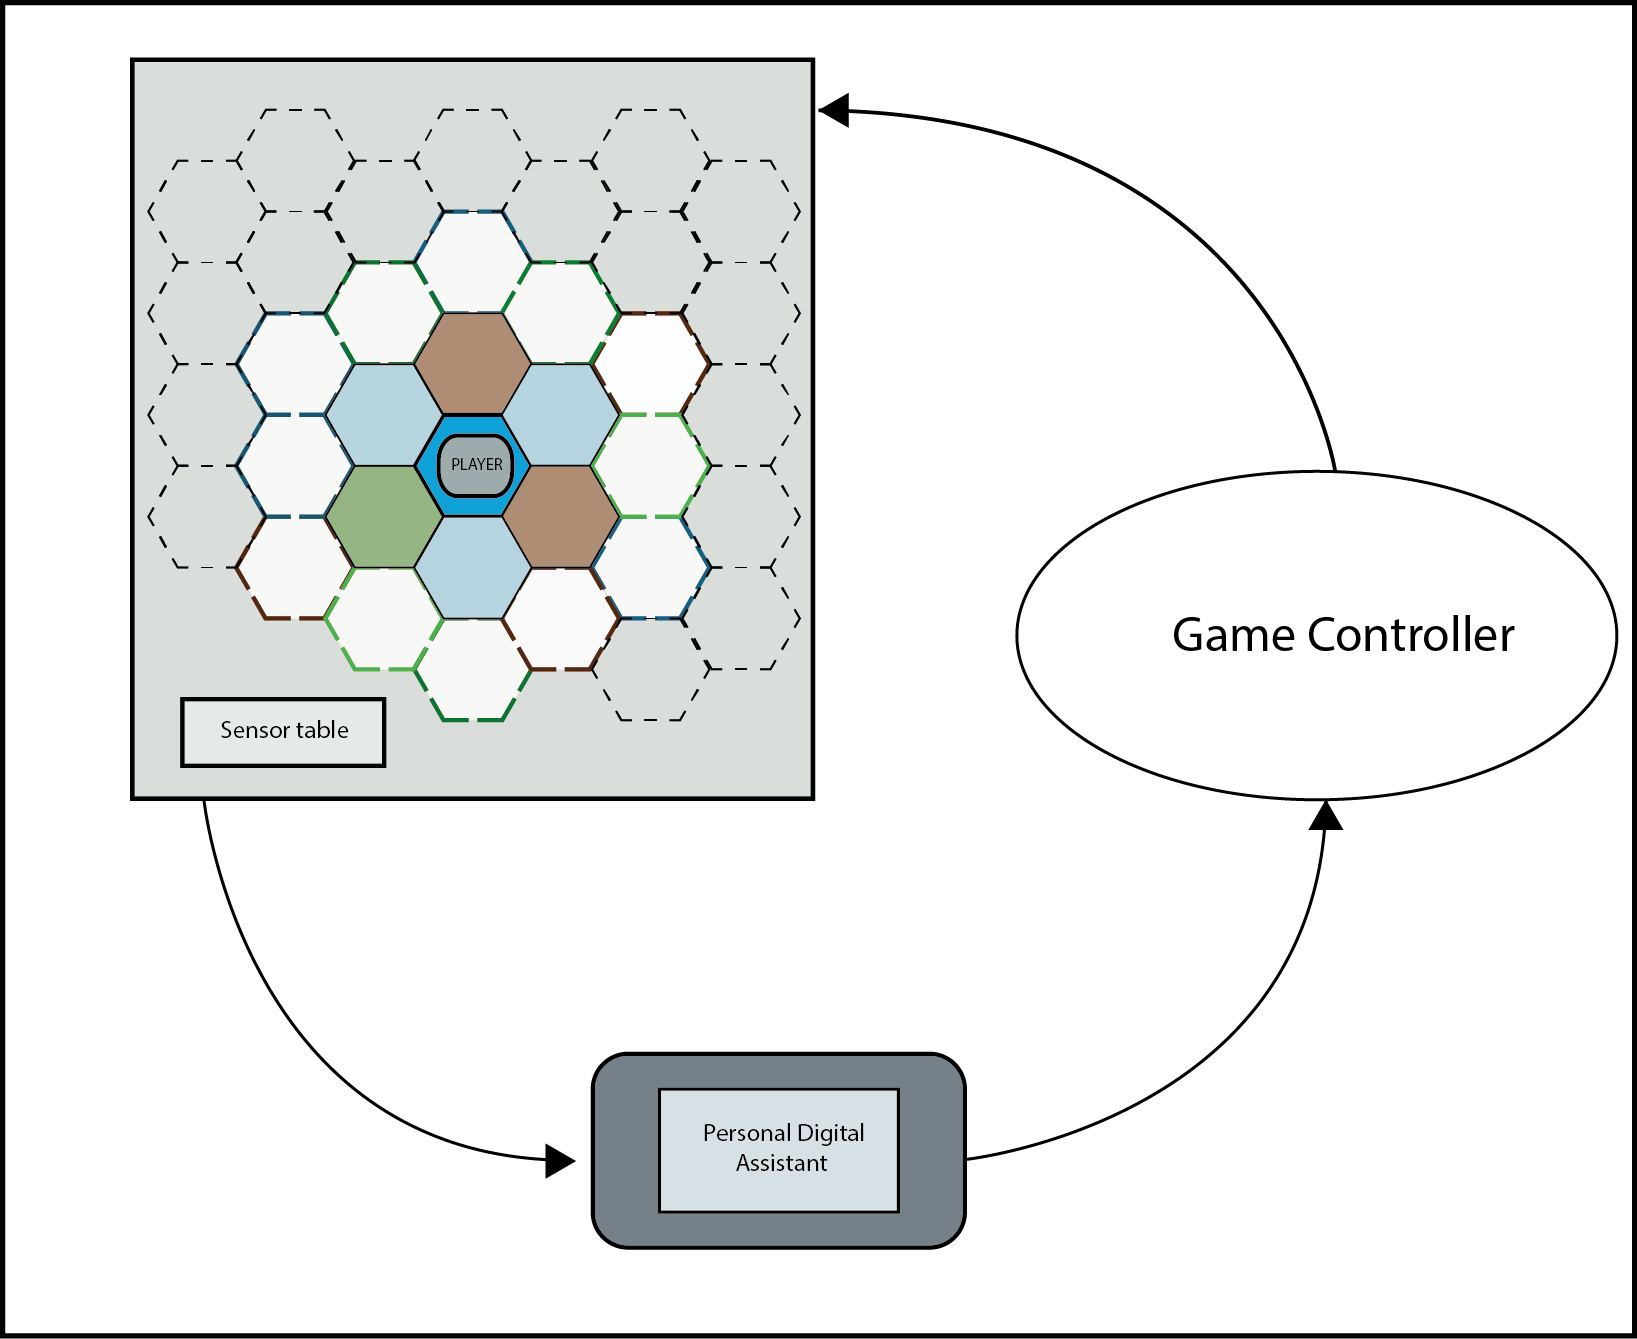
\includegraphics[scale=1]{Images/f_p_fig.png}
    \caption{A representation of \textit{False Prophet}'s set up. A hexagon tiled map is projected on a sensor interface. Only the tiles that are close enough to the players are displayed. The colours represent the different types of terrain they are. The players also have a handheld computer used to display some relevant information. The devices are linked to a game controller that handles the computation required to display the map, or communicate information to the players.}
    \label{fig:falseprophet}
\end{figure}

This experiment was a technical challenge more than a game design experiment. Mandryk and Maranan created a tabletop display using sensors in order to recreate an interface. A tiled map made of 20x30 hexagons is projected on a surface containing infra-red sensors, which can detect the position of the tokens in the displayed tiles. Originally, the hexagon tiles are hidden, except for the one on which the player tokens are placed. It is only when the game's computer detects players moving their tokens that the closest tiles get revealed. The map is linked to a game software that takes care of updating the map, and detect the game pieces. The handheld computers are used to perform actions that cannot be communicated through the game pieces. For example, logic puzzles have to be solved during the game: this is made thanks to the handheld computers, which are also linked to the game controller (see figure\ref{fig:falseprophet}). 

The players are separated in two teams, but the players do not know their team member. The goal of the game is to discover who belongs to which team. To get information about the other players and guess in which team they are, the players move their tokens close to each others. The closer two pieces are, the more detailed the information is. 

The designers were aware of the need to encourage direct communication between the players, and made rules that support such interactions. For instance, direct communication between the different players is not supported by the game system (while this would have been possible thanks to the handheld computers). To exchange clues, the players have to do so verbally, thus forcing them to interact between each other. 

The interest of this experiment is that it tries to exploit the assets of both game boards and computers. First, it uses the context of having an interface around which players can gather and encourages direct communication thanks to certain rules, thus respecting the social nature of tabletop game. Mandryk and Maranan clearly outline their understanding of tabletop games even before entering in the details of the conception of \textit{False Prophets}. Their game is flexible enough so that players can bend the rules if they want to, and they primarily use a board to encourage the interactions between the players, instead of designing it only to transfer information between the player and the game (2002)\cite{art:prophets}.

Second, computation can be used to do complex calculation that would be impossible to do for humans while playing the game. In this case, the manifestation of that is the map that gets revealed dynamically.  While fully analogue games  that possess a similar mechanic, like \textit{Zombies!!!} (T. Breitenstein and K. Breitenstein, 2001)\cite{game:zombies} already exist, the sensor interface could allow many possibilities for game mechanics. This is a typical example of exploiting the digital device, allowing to enable a kind of play experience that is totally new to tabletop games. As a future work, the creators of False Prophets mentioned having "playing pieces that store data, interpret contextual information, and travel continually with the players" The other digital device (the handheld computer) however seems to be thought as a support for all the actions that "cannot naturally be communicated through the game pieces"(2002)\cite{art:prophets}.

By combining the advantages of computation (that is generally used in digital games), and those of board games (allowing a strong interaction between the players), \textit{False Prophets} represents an interesting approach to the genre of hybrid games. It also proves that hybrid games deserve to be thoroughly studied, and that a huge amount of variety can be brought to the world of tabletop games by exploiting digital components.
\subsubsection{\textit{STARS}, the hybrid game platform}
During the Ubicomp '03 conference on ubiquitous computing environment\footnote{"A proposed development of computing in which computers are sufficiently small and inexpensive to be embedded frequently in everyday objects."(Oxford Dictionaries, 2016)}, Magerkurth, Stenzel \& Prante (2003) showed \textit{STARS} \cite{art:stars}, another example of the integration of digital devices in the traditional way of playing tabletop games, though even more complex than \textit{False Prophets}. This project was elaborated as an attempt to show the many possibles interactions between different devices "by realizing computer augmented tabletop games [...] within a smart Roomware® environment" (2003)\cite{art:stars}. In other words, different hybrid games, or adaptations of already existing tabletop games could be played using this platform.
\begin{figure}[h]
    \centering
    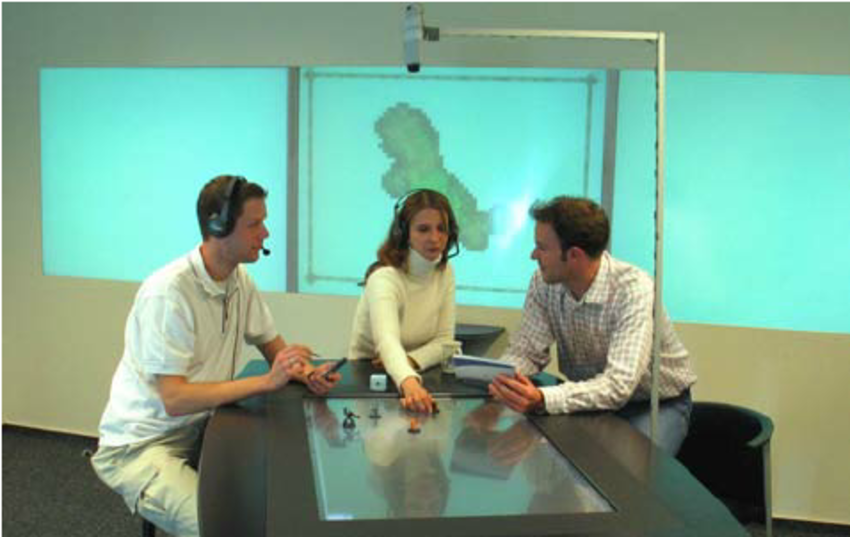
\includegraphics[scale=0.4]{Images/roomware.png}
    \caption{The Roomware® environment used to create \textit{STARS}. The camera detects the position of the different game pieces on the interactive table and. The wall displays are used for public informations and the Personal Digital Assistants for personal, non-shared information. Audio devices are used for communication.}
    \label{fig:roomware}
\end{figure}
The \textit{STARS} platform features an interactive touch-sensitive screen, which displays the content of the game board as well as it manages the interactive playing pieces. A camera is situated over the table and tracks the position of other playing pieces. \textit{STARS} also features a wall display and other digital components like a small Personal Digital Assistant (used by the players to secretly communicate and store personal information related to the game), and audio devices. All the devices are interconnected and managed by a game software (see figure \ref{fig:roomware}). 

Although this experiment looks similar to False Prophets, this multi-device approach is the interest of the project. By exploiting the possibilities offered by the different component of the computing environment, the creators hoped to "go beyond traditional tabletop games, but at the same time preserve the human centered interaction dynamics which makes playing board games a joyful group experience"(2003)\cite{art:stars}. The social dimension of the tabletop game play experience has been used here to prove the efficiency of an interconnected digital environment. The benefits of using such interactive platform has been explained as follows:
\begin{quotation}
Regardless of the number of players involved, playing computer games is still being perceived as a mostly isolated activity. This is due to the interaction being technology centered.[...]The richness of human-to-human interaction
involving eye contact, mimics, and gestures is far from being captured in the purely virtual gameplay of computer games.[...]To further augment the social experience of computer games and facilitate a strong emotional involvement among the players, direct face-to-face interaction should be enabled and new interfaces between the players and the virtual domain must be introduced (Magerkurth, Engelke \& Memisoglu, 2004)\cite{art:stars2}.
\end{quotation}
It could be argued that the statement simplifies too much the interactions between players in digital games, but the approach shows an understanding of the particular relationship between players in a tabletop game. The platform encourages such \textit{computer assisted} interactions, and also opens to the possibility of creating other tabletop games using digital devices as core components, thus enabling new play experiences. Three different game adaptations to the \textit{STARS} platform are described (2004)\cite{art:stars2}.
\begin{itemize}
\item\textit{KnightMage} is a hybrid game that was developed for the \textit{STARS} platform. Its rules are based on classical Hack'n'Slash games\footnote{Term that referred to a type of gameplay in "pen and paper Role Playing Games" such as \textit{Dungeons and Dragons} (Gigax and Arneson, 1974\cite{game:dnd}), before becoming the common denomination of a computer game genre}, in which the players go through dungeons, kill enemies and gather equipment to improve their character and progress through the game. According to its creators, \textit{KnightMage} was designed to "combine the strong social situations of traditional tabletop role-playing games with typical benefits found in computer adaptations of role-playing games" (2004)\cite{art:stars2}. The typical Hack'n'Slash mix of cooperative (fighting the monsters) and competitive (gathering the best loot) gameplay, combined with the physical interactions with the game core components is what enables a new hybrid game play experience based on design patterns extracted from both digital and tabletop game genres.
\item\textit{Candyland}\footnote{Not to be confused with the board game \textit{Candy Land}(Abbott, 1949)\cite{{game:candy}}} was a hybrid game designed for children. The game takes place in a small village that the players can build by placing the components on the tactile table. The game software creates an interactive story based on the children actions. This shows another type of hybrid game model.
\item\textit{Monopoly Adaptation} is based on the classical \textit{Monopoly} (Darrow, 1935)\cite{game:mono}. This experiment is an attempt to show the potential of adapting traditional board games to the \textit{STARS} platform. The adaptation removes the most tedious actions like shuffling cards, managing all the bank notes, and components on the board. To create a new experience, new mechanics made possible thanks to the use of a digital device have been added to the original game. For example, the players can now secretly transfer money to another player in order to form alliances.
\end{itemize}
With a platform like STARS, it could  be argued that the quantity of available information (on the board, the wall display and the Personal Digital Assistant) might get in the way of play by making it too complex. But this invention is interesting in its approach of hybrid board games: it uses the potential of digital devices as core components, enabling new hybrid play experiences that would hardly be possible otherwise.
\subsection{The Hybrid Games market}
The \textit{False Prophets} and \textit{STARS} experiments are early attempts to introduce digital components into tabletop games. However, the complexity of such devices made it very difficult to turn them into a commercially viable product. 
\subsubsection{Development problematics}
As a conclusion of their research, De Boer and Lamers explain the difficulty of developing hybrid games:
\begin{quotation}
The electronic augmentation of board games is still in its infancy. World leading board game manufacturers, although sceptic, are willing to invest resources in the development of such games. Important obstacles are the costs of development and production and the need for game designers to accumulate knowledge on modern technology (De Boer and Lamers, 2004, p.444)\cite{chap:aug}.
\end{quotation}
It is true that hybrid games involve a new type of parallel development between the physical part of the game and the device(s) supporting it and making it hybrid. It involves a transformation of game studios, as well as new possibilities to explore for game designers. An explanation could be that the gap between two industries with few interconnections. This can be noticed in game conventions, where the digital games attract a bigger audience every year while tabletop games are relegated to a small isolated room. This does not mean that playing tabletop games and playing digital games are two incompatible activities; but there is a lack of recognition between the two whereas they are fundamentally based on the same activity: play. This leads to the problem of target audience.

Target audience is an important concept in game design. Not only is it important to know for who the game is made in order to create a product that can be sold on the market, it is also the bases of many design decisions. The approach of hybrid games illustrated by the two experiments shows the lack of a common ground on which to base the games. Saffer describes the thoughts behind a user-centered design with one simple sentence: "users know best" (Saffer, 2010, p.33) \cite{book:id}. This idea could explain why the implementation of digital devices in tabletop games was not popular.  An unclear definition of the target audience, due to the rapidly evolving habits of players regarding digital devices made it hard for designer to focus on a technology to build design decisions.

Primarily, one could think that the main target audience of hybrid games lies in a blurry zone between computer games players and tabletop games players. Tabletop game players are used and attached to the \textit{ritual} (this term can be emphasized because this is exactly how some tabletop game players perceive it) of preparing the board, manipulate physical game components and trying to understand what is the game about before even reading the rules; it is probably the opposite for people playing digital games who are used to learn how a game works, either with a clear step-by-step tutorial, or thanks to in-game (sometimes hidden) clues placed by the designers to understand the game mechanics. Therefore, there is already a problem when designing a hybrid game for the two groups at the same time and the target audience becomes more complex than it seems, and using devices that all the potential players never saw or used before probably did not help when showing the concept to game publishers. This problem was solved by the rapidly increasing popularity of smartphones and tablets.
\subsubsection{A growing interest}
The recent and rapid development and the adoption by a large audience of easily connected devices has provided to developers a natural and heavily supported material on which hybrid game mechanics could be based. Many possibilities are already known by the designers (who probably already possess the devices for their own personal use) and the development of a smartphone or tablet application does not require a very specific programming knowledge (like it was the case for an environment like Roomware®). For that reason, hybrid games have recently started to develop on the market, and could well be a natural evolution for tabletop games if the audience follows.

It has been previously explained in this paper that simple adaptations are not the focus of this paper (though interesting in the way they change the traditional tabletop experience). One thing needs to be mentioned though: those adaptations seem to be what really started the growing interest for digitally enhanced tabletop games. Some games like \textit{Ticket To Ride} (Moon, 2004)\cite{game:ticket} or \textit{Small World} (Keyaerts, 2009)\cite{game:tw}, have seen an surprising increase in the sales of their physical versions, when the digital versions were published on smartphones and tablets for a much lower price(McElroy, 2013)\cite{web:poly}. This proves that the so-called separation between the analogue game target audience and the one of digital games is not as big as expected.

\textit{Zombicide} (Guiton, Lullien and Raoult, 2012) \cite{game:zombi}, seems to be one of the first innovative examples to implement digital components to enhance the tabletop experience. Designers rapidly saw the interest of the experience:
\begin{quotation}
The app maximizes gameplay by virtualizing the mundane aspects, like dice rolls and card shuffles, and allows players to focus their energy on strategizing their next move. You can play the game without the app, but doing so is like wandering into a zombie-infected street without a shotgun or machete (Flaherty, 2012)\cite{web:wired}.
\end{quotation}
The fact that \textit{Zombicide} can be played without the application makes the game fall out of the definition of \textit{hybrid games} (the digital device is not a core component in that case). However, the success proved the commercial potential of such design, and others followed in its steps.

\begin{figure}[h]
    \centering
    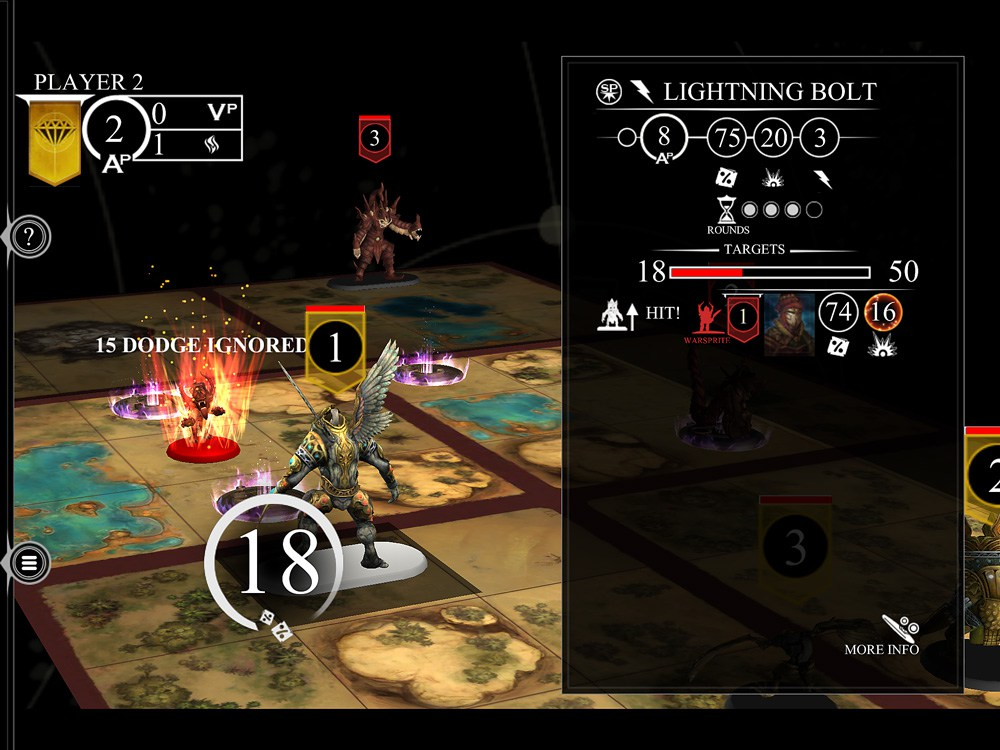
\includegraphics[scale=0.2]{Images/golem_app.jpg}
    \caption{The resolution of the fights in \textit{Golem Arcana} as they are displayed on the app}
    \label{fig:Golem}
\end{figure}

\textit{Golem Arcana} (Harebrained Schemes, 2014)\cite{game:golem} is often cited as one of the most innovative recent example of tabletop game experience enhancement through the implementation of a digital device (Banks, 2014)\cite{web:golem}. It is a battle between to players, based on miniatures that are moved on the board. This case is particular though: the game uses a Bluetooth stylus to recognize the pieces that are used on the board, in order to transmit the informations to the application. When a battle between two golems occurs, the players can choose between rolling dice and calculate the damages, or let the application do all the maths. The mechanic itself is not dependent on the digital device, but the experience is greatly improved by the fun of  "tapping your target with the stylus and then turning to your phone or tablet and watching as hit points disintegrate from your target" (Banks, 2014)\cite{web:golem} (see figure \ref{fig:Golem}). However, the whole game cannot be played without digital devices: the application is used to chose between different scenarii, which declares how the board must be set up at the beginning of a game. Moreover, the game rules are explained through the devices, which is cited as an advantage that makes the game very accessible.

All these examples prove the development of the hybrid game genre. The games have evolved from simple adaptations of existing games that have attracted the attention of a wider audience, to games that use the digital devices to enable a new experience. 
\subsubsection{Playing a Hybrid Game - \textit{XCOM: The Board Game}}
This overview of the hybrid game market will be concluded by a play-through analysis of a hybrid game as defined in this paper: a board game that uses a digital core component to enable a new kind of play experience. This has been done while developing Archipelago, in order to understand the impact of such an implementation.

For the majority of players, X-COM (sometimes written "XCOM") is a series of video games which first episode was \textit{UFO: Enemy Unknown}\cite{game:xcom} (Microprose, 1994)\footnote{Also known as \textit{X-COM: UFO Defense} in its north-American version.}. The series has many episodes and spin-off, and also a tabletop game plainly called \textit{XCOM: The Board Game} (Lang, 2015)\cite{game:xcomtbg}.
\begin{figure}[h]
    \centering
    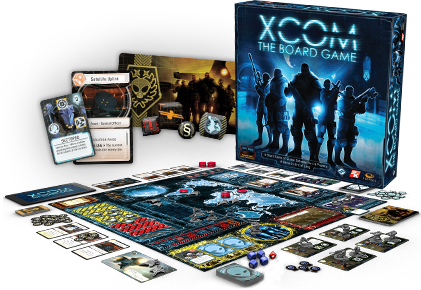
\includegraphics[scale=0.5]{Images/xc01_layout.png}
    \caption{The content of \textit{XCOM: The Board Game}}
    \label{fig:XCOMBG}
\end{figure}
What makes this game interesting for the purpose of this paper is its use of a digital component: an application which has to be downloaded on a digital device (smartphone, tablet or computer) (see figure \ref{fig:XCOMBG}) or opened in a web browser. The game simply cannot be played without this application, since it displays instructions that the players have to follow. On a certain extent, it cannot even be learnt without it: in the box, only a very short leaflet explains how to set up the game and where to find the application. The rules book is not included in the package - which can be disturbing for some players. Instead, all the rules are explained during the - optional - tutorial phase explaining the flow of the game, step by step. 

The game is described as a one to four players cooperative game. However, since the players share the same interest and goal, the game actually falls the definition of collaborative games that has been previously explained in this paper. Therefore, this is how the game is going to be referred as from now on.

In \textit{XCOM: The Board Game}, the players are part of the \textit{X-COM}, a paramilitary organization that defends the Earth against an alien invasion, after all the regular armies have failed to do so. The game's board is a representation of a world map, with other boxes used for the different game mechanics.

Fist of all, there are several levels of difficulty available. It must be selected prior to starting the game. The level of difficulty affects in various ways the instructions given by the application integrated in the game.

\begin{figure}[h]
    \centering
    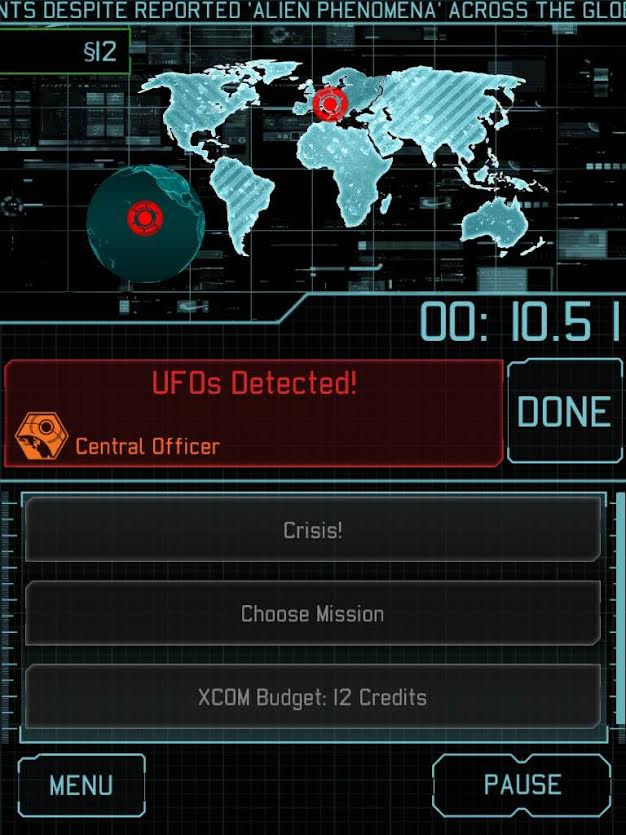
\includegraphics[scale=0.3]{Images/xcom_boardgame_app.jpg}
    \caption{Instructions displayed by the app during the timed phase}
    \label{fig:XCOMAPP}
\end{figure}


One round is divided in two phases: the Timed Phase and the Resolution Phase. The companion application tells the players the order of the different tasks that constitute one phase, as well as how much time is available to finish it - knowing that the order of the tasks changes over the rounds (see figure \ref{fig:XCOMBG}). The tasks are a preparation for the resolution phase: the players discuss to allocate resources in the best possible way, assign soldiers to defend the \textit{X-COM} base, or prepare to repel the next alien attack. The players also have missions to solve, which are a good way to get more resources. There is also a final mission that the players have to complete in order to finish the game. As its name suggests, the players have limited time to perform the tasks during the Timed Phase, but there is a Pause button in case the players need more time to think about the best way to perform the tasks. In the normal and higher difficulty modes, the time during which the game can be paused is limited but is renewed at the beginning of each round.

During the Resolution Phase, the players solve the tasks they have prepared during the Timed Phase. This often takes the form of dice rolls. The tasks to solve are different depending on the player's role. At the end of the Resolution Phase, the player responsible for managing the digital device is asked to enter a few information about the round (i.e. what is the current panic level of panic for each continent and if a mission as been successful or not). These inputs are necessary for the application to generate the locations where the aliens will spawn during the next turn. Four roles must be split between the players (they can have more than one role in case of a game with less than four players):
\begin{itemize}
\item The Central Officer is the only player that has to use the digital device, she has to relay the instructions that are displayed on the application to the other players. Also, the Central Officer is responsible for placing the alien tokens at the right on the game's board when instructed by the application. She can also decide when to use the pause button to give more time to her team.
\item The Chief Scientist researches alien technologies when instructed by the Central Officer (relaying the instructions given by the application), which are bonuses that help the other players (or the Chief Scientist herself) performing their tasks.
\item The Squad Leader controls the ground soldiers. This is done to defend the base when it is attacked, and when trying to solve one of the missions. The dead aliens are used as a resource by the Chief Scientist to develop new technologies.
\item Performing tasks cost money. The Commander is the player responsible for the budget, and thus manages an overall strategy. She also deals with the UFO that are spawned all over the world. If one of the continent is not defended correctly, its panic level increases, and it becomes even harder to defend. When two continents have reached the maximum panic level, the game is lost.
\end{itemize}
\textit{XCOM: The Board Game} definitely shows how the use of a digital device can enable interesting playful experiences. The fact that the Timed Phase is indeed limited in time is not an absolutely new feature in itself. But once the available time to perform a task is up, the next task starts directly and the players have to abandon what they were doing and move on in order to keep up with the application. Because of this, playing as the Chief Officer nicely recreates a feeling of being the one without whom the team would be overwhelmed by the flow of the game. The instructions coming from that player have then to be clear, and quick. The combination of the time limit with the random order in which the tasks have to be performed creates a feeling of constant emergency during the Timed Phase. Succeeding in performing all the tasks in due time, feels relieving and rewarding, as the team coordination is working correctly. Players learn how to rest on their team members while doing their best not to fail. This model of team dynamic would hardly be possible to recreate without the use of the digital device, because of the number of game pieces that would be required to simulate it. Here, the device simply uses a combination of some of its basic functions, and some player inputs. The simplicity enables an experience that would be impossible without a digital component. Therefore, the game deserves its status of \textit{hybrid game}.

Aside from what it brings to the play experience, the way the application is used to teach the game is also interesting. Traditional rulebooks usually follow a step-by-step process as well. But the application encourages the players to perform all the actions one by one, while the explanations are displayed. This make the rule learning phase very similar to strategy video game tutorials, where the players are encouraged to use a unit to learn its potential. This combined with the collaborative game play, where smaller tasks are divided between players makes it very easy to learn how the game works. It is not surprising that the game can then be won without even knowing exactly what the other players had to do.

The device is normally not too intrusive in the game, as reading the instructions fast and clearly is part of the experience. The only aspect that interferes with the experience being the moment when the player holding the device has to enter some inputs, so that the information about what happened during the turn can be filled to the device. Nonetheless - because it is an uncommon component to use in a tabletop game - not having to do anything with the device itself can feel a bit frustrating for some players. A last detail is also worth noticing when analysing a hybrid game like this: the game flow can be completely annihilated if the device runs out of battery - which can be very frustrating when playing a tabletop game. 
\subsection{Procedural Content Generation}
To design Archipelago, it has been decided to use PCG in order to explore hybrid game mechanics. To understand what this implies in terms of technology, design and development, a description of the technical concept, as well as its common uses in game design will be provided in the following paragraphs.
\subsubsection{A content creation method}
\begin{quotation}
"Procedural content generation (PCG) refers to the algorithmic creation of content. It allows content to be generated automatically, and can therefore greatly reduce the increasing workload of artists." (Rolan van der Linden, et al., Procedural generation of dungeons, March 2014). \cite{art:pcg}
\end{quotation}
This quote tells us that PCG does not really have anything to do with the playing of the game it self, rather the contents within it, hence the name procedural \textit{content} generation. 
However, it is not always as simple as that. The line between when the content is being generated by the user and what is generated through assisting the user is fuzzy.
As an example from \textit{What is Procedural Content Generation? Mario on the borderline}\cite{art:whatpcg}, the players interaction with the game \textit{Sim City}, generates more content indirectly based on the interactions. This kind of can be described as Computer Assisted Design. As explained however, there is a very thin line between when the game ends and the algorithms start. 

The place where the line get blurry is when the algorithms generate content based on human input. The reason it is a grey area is because it enters the region of computer assisted design(CAD)\cite{book:cad}.
It is becoming more accepted within larger companies, as a way to lighten workload of other artists, and its uses range between various fields.
To build on what R. van der Linden, et al. say in their paper, about reducing workloads, PCG is a great tool to create templates for content, based on data from designer, artists, etc. PCG can also be used as a tool for aiding in creating content.  
The general idea behind this is that a tool generates some content or usable structure, which it then exposes to a designer. The designer can tweak parameters and sometimes directly interact with the generated content. This way a designer might be presented with a basic structure of a tree, and then have the ability to add branches and leaves, which are in turn generated by the tool. 
The work of the artist is aided by the computer, giving the artist more time to work out the details. Computer generates templates and a base, then it is up to the artist to look over the content and see whether it is pleasing enough, fun enough, and/or acceptable in the final form. The final idea behind this is that it is in the minds of humans that creativity lies. 

PCG allows to generate more content without putting more effort into the manual work in order to populate one's virtual world. With pcg you can design the template and rules you want in order to generate a wide range of items for your game, without having to design each individual item or use copies of the same few items. An example is the application is the tool called \textit{SpeedTree}. This application allows for the generation of different tree which can be used in the environment without having the feel of a copy paste environment. In this PCG allows the designers to focus on creating interesting game play and environments and leaves the details of the individual structures to the pcg tool. 

PCG can also be used to generate a larger play space, by allowing for near infinite variations and/or generations, the replay experience is varied enough to allow for greater replayability in total. Games such as \textit{Age of Empires} and \textit{Civilization} are well known for their map generation, creating playable and enjoyable maps, each different from the last.


Other aspects within the PCG world, which is becoming more and more accepted and used, is "Experience Driven" PCG\cite{art:exppcg}. This concept is taking into account the previous events and data gathered within the game or application. By using gathered data, the newly generated contents can be altered to better fit with the way the previous content was used. Say you have a map in a first person shooter (FPS), and the initial map was generated statically by PCG, and not by E.D.PCG. The first map could be a very good one, by all means, but the program has no way of actually knowing how it will be used. Then by gathering data from an actual live run of the program, the PCG algorithm can then be altered to take into account frequent patterns that may occur, what open areas are most used, places with high chance of death, etc. Basically by combining some form of data mining with PCG and have a clever way of integrating them based on experience, you get a smarter way of generating content, and the content will have more \textit{meaning} as it is in fact based on real life events and occurrences.

\subsubsection{Experience-Driven PCG}
\begin{quotation} 
"Experience-Driven Procedural Content Generation (EDPCG) defines a novel approach to PCG. [...] We view game content as building blocks of games, and games as potentiators of player experience. Therefore, content can be seen as indirect building blocks of player experience [...]" (Yannakakis and Togelius, 2011) \cite{art:edpcg}
\end{quotation}

The purpose of EDPCG is to generate "building blocks" that can be modelled to the players playing the game, and to generate blocks of the game that is built up by preceding results and analysis. Generating content that is based on a model of the player experience and how the player interacts with the game, can arguably be called Player-Experience-Driven PCG, whilst EDPCG as a wider term can be any content that is generated by usage of experience and \textit{already generated} content. Usually EDPCG is done by analysing the player's reactions, behaviour, and frequent occurrences and creating models based on the collected data. By doing this, you can elicit the player experience, and create models that utilized these properties. How these models are used, depends on the contexts of what the games are trying to create. If the game is meant to be as frustrating as possible, the models might want to be adjusted to bring forth behaviour and reactions with the players that matches the criteria found within the analysis. The same concept goes for other experiences as well, i.e. sadness, joy, etc.

In this thesis, the more likely approach will be to look at a looser term of EDPCG, as this will be more suited for time scope available.
Another reason for this decision is the fact that this will be a hybrid game, both a physical game and a digital game combined, which means that there will be much more emphasis on the player-to-player-interaction in the physical part of the game, than what it would if it was purely a digital game. Other thoughts behind the use of EDPCG in this thesis, is to generate content to the players, that will influence "how" the game is played, \textit{how} the players interact with each other, and \textit{what} the players feel they get out of the game, in terms of joy, excitement, frustration, etc. 
The version of \textit{Experience}-Driven PCG thought of here, is also thought to be able to show the difference between having only a board game, versus that of having a digital application integrated into the game, and give the players the experience of \textit{history} in a board game, and \textit{consequences} of actions.

\subsubsection{L-Systems}
A Lindenmayer system, or L-System in short, is a PCG algorithm which is based on grammars and rules. In the start, you have an axiom, usually a simple string, which is the initial value that the system will expand upon, along with rules/grammar that explains what within the axiom needs to be changed over each iteration. The algorithm also needs a number for how many times the axiom will be changed; the iteration number. What this algorithm does, if you for example are going to be using a string and expand upon that, is to go through each element i.e. the characters, that is found within the string, check for matching rules to each given character, and then apply the result of said rule to the result string.
What this leaves us with, is a larger expanded string, that has been rebuilt in accordance to the rules that goes with it. This algorithm allows for quick generation of a larger connected outcome, that when interpreted afterwards, can be used in a multitudes of ways. It is a good way to generate maps, dungeons and levels, and it can also be used to create contents within dungeons at the same time. If a rule consists of a marker for a puzzle with its challenge and reward, the interpretation part can hold the code for how to place those objects. 
Overall, the L-System allows for rapid generation of greater "summarized" data, and it is then up to the interpretation part to create and use the data to its advantage.
It can be used in both 2D as well as 3D environments, all depending on the interpretation of the generated result. A common way to distinguish between dimensions is to have various special characters specifically assigned to movement and orientation in the 3D space, e.g. '-' and '+' for orientation around the z-axis, '$\&$' and ' $\wedge$ ' for the y-axis, and '/' and '$\backslash$' for the x-axis. In 2D solutions, however, it is most common to only utilize '+' and '-'. 

\subsubsection{Procedural Content Generation in Game Design}
PCG being a programming concept allowing the rapid creation of content, it has been mostly used for video games. There are counter examples to that statement though. In films for example, PCG can be used to rapidly generate complex scenes. The battle scenes in \textit{The Lord Of The Rings: The Two Towers} (2002)\cite{film:lotr2} and its sequel \textit{The Lord Of The Rings: The Return of the King} (2003)\cite{film:lotr3} for example have been made possible thanks to an agent generator software called \textit{Massive} (Regelous, n.d)\cite{soft:massive}, which procedurally generates intelligent and independent agents in order to simulate large-size battles. This paper will leave that case aside though and focus in the next paragraphs on PCG-based games in order to point out the game design concepts that are enhanced thanks to the use of PCG. The basic concepts have been identified by researchers (Smith et al., 2011)\cite{art:pcgbased}.

The most obvious aspects reinforced by PCG that are pointed out in this article are "replayability" and "adaptability", which are considered interconnected.

"Replayability" is a concept used to describe the fact that a player can still discover new aspects of a game even after finishing it the first time. The paper refers to the game \textit{Rogue} (Toy, Wichman and Arnold, 1980)\cite{game:rogue}, as one of the earliest and most famous example of PCG-based games. The basic concept of \textit{Rogue} is simple and has given birth to a new game genre - also giving it its name: \textit{Rogue-like games}. The principle of Rogue-like games is the following: the player explores his environment (a dungeon in the case of \textit{Rogue}), collects items (like equipment) to become stronger and defeat more and more dangerous enemies. In Rogue-like games, the environment (and thus the collectible items and the enemies) are procedurally generated which ensures that the players are really unlikely to face the same situation several times when going through the game. This shows how PCG can enhance the replayability of a game.

In the same study, "adaptability" is referred as "the use of procedural content generation to adjust content in reaction to player actions or skill levels". An example can be found in the video game \textit{FTL: Faster Than Light} (Subset Games, 2011)\cite{game:ftl}. This game - which uses Rogue-like game mechanics - is based on procedurally generated events that players   have to overcome, sometimes by choosing between two different solutions. The selected option will then influence the next events generated by the game. In that case, the player's actions are the parameters used by the algorithm to generate the content. In other words the game content adapts itself to the player's action.

A distinction is also made between "PCG systems augment traditional mechanics and those which enable new mechanics entirely" (2011, Smith et al.). That distinction is made to differentiate the impact of PCG on the game's mechanics and the effect on the play experience. The example of \textit{Borderlands} (Gearbox Software, 2009)\cite{game:border} is given in the paper to demonstrate that PCG does not change the core mechanics of the game itself - a first-person shooter game in which the players collect more and more powerful procedurally generated weapons. However, the play experience is vastly affected by the perceived randomness that PCG can enable. The excitement when waiting for the containers holding weapons, or the sudden burst of adrenaline when a powerful weapon appears could not be reproduced without the use of PCG. The Game Designers seem to have also enhanced that aspect in the multi-player mode by making the generated items collectible by any player, even players that have never taken part in the battle (this mechanic is generally called "ninja-loot"). Another example that comes to mind is the game \textit{Diablo} (Blizzard North, 1996)\cite{game:diablo}. It uses the same approach to procedurally generate equipment, but the emphasis is put on the optimization of the character's attributes and skills. This use of PCG is opposed to game mechanics based on PCG: \textit{Galactic Arms Race} (Evolutionary games, 2010)\cite{game:gar} uses a mechanic in which the more a weapon is used, the more the chances of getting a weapon having similar properties increase. This mechanic is used to base the gameplay on the player's choices, as it becomes important to use the weapons with the preferred attributes, in order to get similar weapons later in the game. In that sense, the mechanic can be considered PCG-based.

Finally, this mechanic also illustrates the last aspect of PCG-based Game Design described in the article, which is the player's control over the game's content. This means that the player has an influence over the PCG system in the game. In theory, the players input are often used by the algorithm to use the new content, so the influence of the player is real. However, in order to have a certain control over the game's content, a player must be aware that she influences the algorithm with her choices. This is what is called "direct control" (Smith et al., 2011). It is opposed to indirect control, when a player's actions are taken into account when the games generating the content without her knowing in what extent the actions have influenced the content generation. This is the model which is used in the majority of PCG-based games. This shows an interesting aspect of using PCG for designing games: PCG can help creating a feeling of surprise (by simulating randomness) as well as it can be used to show the player that her actions influenced the game in some way, thus creating a feeling of responsibility and sometimes even guilt.
\\\\
PCG is a tool that has several benefits. It allows the rapid creation of content, which means less work load for artists. It also allows to use data relative to the player's input in the game, in order to generate relevant content in some case. This allows for designing mechanics enabling interesting experiences for designers. Implementing such mechanics as a core element in tabletop games would then greatly modify the play experience in various way. However, because the concept of hybrid games is relatively new, this design space needs to be explored.
\subsection{Game Design Methods}
As a conclusion of the framework on which Archipelago was based on, a brief description of different design concepts that are important to understand the purpose of the project have to be described. The list is of course not exhaustive and other concepts have been used during the project. The ones that have been chosen here show the experimental aspect of the game.
\subsubsection{Iterative design and prototyping}
The development of a game - analogue or digital - is made thanks to several iterations. These iterations take the form of prototypes, each of them exploring a design space, or the combination of several designed elements. Houde and Hill explain the use of prototypes in design:
\begin{quotation}
Prototypes provide the means for examining design problems and evaluating solutions. Selecting the focus of a prototype is the art of identifying the most important open design questions. If the artifact is to provide new functionality for users - and thus play a new role in their lives - the most important questions may concern exactly what that role should be and what features are needed to support it. If the role is well understood, but the goal of the artifact is to present its functionality in a novel way, then prototyping must focus on how the artifact will look and feel. If the artifact’s functionality is to be based on a new technique, questions of how to implement the design may be the focus of prototyping efforts (Houde and Hill, 1997, pp.1-2)\cite{book:proto}.
\end{quotation}
This statement sums up the philosophy behind prototyping: prototypes are not an early version of a design that is made to be polished towards its final state. Each iteration has a testing purpose, as well as a communicative aspect for the development team. In the case of a game development, this can take several form.


\subsubsection{Interaction design}

